\documentclass[12pt,a4paper]{report}

\usepackage[utf8]{inputenc}
\usepackage[english]{babel}
\usepackage{amsmath}
\usepackage{amsfonts}
\usepackage{amssymb}
\usepackage{graphicx}
\usepackage{cite}
\usepackage{hyperref}
\usepackage[left=2cm,right=2cm,top=2cm,bottom=2cm]{geometry}


\author{Josep Puig}
\title{Renting an existing Ground Station}


\begin{document}
\maketitle


\chapter{Contact with existing Ground Stations}

Some companies that own a Ground Station have been contacted in order to get some information about costs and conditions of renting their stations. Nevertheless, no answer has been received yet, and no information is easily found on the Internet. 

Therefore, in order to characterize the costs of renting a Ground Station, it has been decided to use LeafSpace. 

\chapter{LeafSpace}
LeafSpace is an italian company which provides a ground stations network, specifically designed to exchange data with micro and nanosatellites in a fast and simple way. Their global distribution ensures a high visibility time for a wide range of orbits, allowing their customers to download massive amounts of data. 

This means that LeafSpace lets customers use their Ground Stations to download data, but does not permit to rent them in exclusive, which is the main idea of this project. Due to the small amount of information existing, LeafSpace will be considered in order to get a first approximation and to develop an OWA to decide. 

\section{Features}
\subsection{Antenna}
LeafSpace allows to receive data from VHF (137-144 MHz), UHF (400-402 MHz), S-Band (2.2-2.4 GHz) and X-Band (8.025-8.5 GHz), but only can transmit UHF (401-403 MHz) and S-Band (2.025-2.11 GHz). The polarization is RHCP/LHCP (Right and Left Hand Circular Polarization, respectively). The moduation and the protocol are totally configurable. The datarates depend on the bandwidth: for UHF, up to 100 Kbps; for S-Band, up to 30Mbps; and for X-Band, up to 100Mbps. 

\subsection{Pricing}
The prices, expressed in euros/Mbyte, depend on the bandwidth too: for receiving, VHF 5, UHF 5, S-Band 0.4 and X-Band 0.1, while for transmitting it is UHF 20 and S-Band 2 (recall that they can only transmit in those two bandwidths). 

Nevertheless, it is also stated that customized subscriptions are available for missions with large data transfers and constellations. Then, it is highly probable that a better pricing can be achieved. 

\subsection{Boost Performance}
Within 2017, 20 Ground Stations are scheduled to be implemented all around the World, ensuring a telecommunication service with a considerable increase of visibility time, together with a drastic reduction of communication latency for a wide range of Low Earth Orbits. 

\subsection{Way of use}
Data management is achieved with a user-friendly web-based interface, along with cloud storage granting direct access to download data at any time. 

Since this is all granted by LeafSpace, there would be no need to develop the Ground Segment discussed before. 

\subsection{Services}
It is claimed to be 24/7 full availability of downloaded data, API access for constellations management, full redundant cloud storage for up to 10 days, advanced levels of data encrypting on demand, automatic scheduling, upling and downling, ranging and tracking, and 24/7 alert service. 

\subsection{Map}
In the following image there is the planification of Ground Stations to be built in the following years by LeafSpace. 

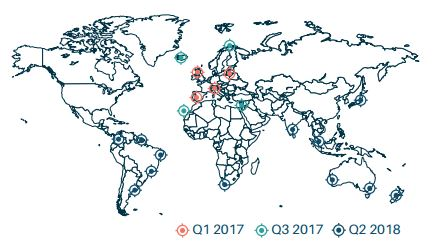
\includegraphics{LeafSpace.jpg}

\subsection{Operation}
No information relative to operation is given. It is certainly stated that its working way is automatic. Despite so, some maintenance is surely required, though its cost is probably low.




\end{document}
